\documentclass[
11pt, % The default document font size, options: 10pt, 11pt, 12pt
%oneside, % Two side (alternating margins) for binding by default, uncomment to switch to one side
english, % ngerman for German
singlespacing, % Single line spacing, alternatives: onehalfspacing or doublespacing
%draft, % Uncomment to enable draft mode (no pictures, no links, overfull hboxes indicated)
%nolistspacing, % If the document is onehalfspacing or doublespacing, uncomment this to set spacing in lists to single
%liststotoc, % Uncomment to add the list of figures/tables/etc to the table of contents
%toctotoc, % Uncomment to add the main table of contents to the table of contents
%parskip, % Uncomment to add space between paragraphs
%nohyperref, % Uncomment to not load the hyperref package
headsepline, % Uncomment to get a line under the header
%chapterinoneline, % Uncomment to place the chapter title next to the number on one line
%consistentlayout, % Uncomment to change the layout of the declaration, abstract and acknowledgements pages to match the default layout
]{lmu_thesis} % The class file specifying the document structure

\usepackage[utf8]{inputenc} % Required for inputting international characters
\usepackage[T1]{fontenc} % Output font encoding for international characters

\usepackage{mathpazo} % Use the Palatino font by default

\usepackage[backend=bibtex,style=numeric,sorting=none,natbib=true]{biblatex} % Use the bibtex backend with the authoryear citation style (which resembles APA)

\addbibresource{reference.bib} % The filename of the bibliography

\usepackage[autostyle=true]{csquotes} % Required to generate language-dependent quotes in the bibliography

%----------------------------------------------------------------------------------------
%	MARGIN SETTINGS
%----------------------------------------------------------------------------------------
\usepackage{amsmath,amsfonts,stmaryrd,amssymb} % Math packages

\usepackage{enumerate} % Custom item numbers for enumerations

%\usepackage[ruled]{algorithm2e} % Algorithms

\usepackage[framemethod=tikz]{mdframed} % Allows defining custom boxed/framed environments

\usepackage{listings} % File listings, with syntax highlighting
\lstset{
	basicstyle=\ttfamily, % Typeset listings in monospace font
}
%\setlength{\mathindent}{3pt}
\usepackage{bbold}
%\usepackage{cite}
\usepackage{hyperref}
\usepackage{physics}
\usepackage[overload]{empheq}
\usepackage{tikz}
\usepackage{tikz-3dplot}
\usetikzlibrary{3d,calc}
\usetikzlibrary{mindmap,trees,backgrounds}
\usepackage{caption}
\usepackage{subcaption}
\usepackage[most]{tcolorbox}
\usetikzlibrary{math}
\usepackage{ifthen}
%\usepackage[active,tightpage]{preview}
%\PreviewEnvironment{tikzpicture}
%\setlength\PreviewBorder{1pt}
\usepackage{geometry} % Required for adjusting page dimensions and margins

\geometry{
	paper=a4paper, % Change to letterpaper for US letter
	inner=2.5cm, % Inner margin
	outer=3.8cm, % Outer margin
	bindingoffset=.5cm, % Binding offset
	top=1.5cm, % Top margin
	bottom=1.5cm, % Bottom margin
	%showframe, % Uncomment to show how the type block is set on the page
}
%\usepackage[backend=bibtex,style=authoryear,natbib=true]{biblatex}
%\usepackage[longnamefirst]{natbib}
%\addbibresource{reference.bib}
%----------------------------------------------------------------------------------------
%	FONTS
%----------------------------------------------------------------------------------------

%\usepackage[utf8]{inputenc} % Required for inputting international characters
%\usepackage[T1]{fontenc} % Output font encoding for international characters

\usepackage{XCharter} % Use the XCharter fonts

\thesistitle{Constraints on The Infinite Distance Limit Under Renormalization Group} % Your thesis title, this is used in the title and abstract, print it elsewhere with \ttitle
\supervisor{} % Your supervisor's name, this is used in the title page, print it elsewhere with \supname
%\examiner{} % Your examiner's name, this is not currently used anywhere in the template, print it elsewhere with \examname
\degree{Master of Physics} % Your degree name, this is used in the title page and abstract, print it elsewhere with \degreename
\author{Shun \textsc{Miyamoto}} % Your name, this is used in the title page and abstract, print it elsewhere with \authorname
%\addresses{} % Your address, this is not currently used anywhere in the template, print it elsewhere with \addressname

\subject{Physics} % Your subject area, this is not currently used anywhere in the template, print it elsewhere with \subjectname
\keywords{} % Keywords for your thesis, this is not currently used anywhere in the template, print it elsewhere with \keywordnames
\university{\href{http://www.university.com}{University Name}} % Your university's name and URL, this is used in the title page and abstract, print it elsewhere with \univname
\department{\href{http://department.university.com}{Department or School Name}} % Your department's name and URL, this is used in the title page and abstract, print it elsewhere with \deptname
\group{\href{http://researchgroup.university.com}{Research Group Name}} % Your research group's name and URL, this is used in the title page, print it elsewhere with \groupname
\faculty{\href{http://faculty.university.com}{Faculty Name}} % Your faculty's name and URL, this is used in the title page and abstract, print it elsewhere with \facname

\AtBeginDocument{
\hypersetup{pdftitle=\ttitle} % Set the PDF's title to your title
\hypersetup{pdfauthor=\authorname} % Set the PDF's author to your name
\hypersetup{pdfkeywords=\keywordnames} % Set the PDF's keywords to your keywords
}
\begin{document}

\frontmatter % Use roman page numbering style (i, ii, iii, iv...) for the pre-content pages

\pagestyle{plain} % Default to the plain heading style until the thesis style is called for the body content

%----------------------------------------------------------------------------------------
%	TITLE PAGE
%----------------------------------------------------------------------------------------

\input{chapters/title}
%----------------------------------------------------------------------------------------
%	DECLARATION PAGE
%----------------------------------------------------------------------------------------

\begin{declaration}
%\addchaptertocentry{\authorshipname} % Add the declaration to the table of contents
\noindent I hereby declare that this thesis is my own work, and that I have not used
any sources and aids other than those stated in the thesis.

%\noindent I, \authorname, declare that this thesis titled, \enquote{\ttitle} and the work presented in it are my own. I confirm that:

%\begin{itemize} 
%\item This work was done wholly or mainly while in candidature for a research degree at this University.
%\item Where any part of this thesis has previously been submitted for a degree or any other qualification at this University or any other institution, this has been clearly stated.
%\item Where I have consulted the published work of others, this is always clearly attributed.
%\item Where I have quoted from the work of others, the source is always given. With the exception of such quotations, this thesis is entirely my own work.
%\item I have acknowledged all main sources of help.
%\item Where the thesis is based on work done by myself jointly with others, I have made clear exactly what was done by others and what I have contributed myself.\\
%\end{itemize}
\vspace{4cm}
 
\hspace{2cm} Place, Date \hfill Signature \hspace{2cm}

\end{declaration}

\cleardoublepage


%----------------------------------------------------------------------------------------
%	ABSTRACT PAGE
%----------------------------------------------------------------------------------------

%\input{chapters/abstracts}

%----------------------------------------------------------------------------------------
%	ACKNOWLEDGEMENTS
%----------------------------------------------------------------------------------------
\begin{acknowledgements}
    \addchaptertocentry{\acknowledgementname} % Add the acknowledgements to the table of contents
    %The acknowledgments and the people to thank go here, don't forget to include your project advisor\ldots
    I first of all would like to express ..
    \end{acknowledgements}


%----------------------------------------------------------------------------------------
%	LIST OF CONTENTS/FIGURES/TABLES PAGES
%----------------------------------------------------------------------------------------

\tableofcontents % Prints the main table of contents

\listoffigures % Prints the list of figures

%\listoftables % Prints the list of tables

%----------------------------------------------------------------------------------------
%	ABBREVIATIONS
%----------------------------------------------------------------------------------------

%\begin{abbreviations}{ll} % Include a list of abbreviations (a table of two columns)

%\textbf{LAH} & \textbf{L}ist \textbf{A}bbreviations \textbf{H}ere\\
%\textbf{WSF} & \textbf{W}hat (it) \textbf{S}tands \textbf{F}or\\

%\end{abbreviations}

%----------------------------------------------------------------------------------------
%	PHYSICAL CONSTANTS/OTHER DEFINITIONS
%----------------------------------------------------------------------------------------

%\begin{constants}{lr@{${}={}$}l} % The list of physical constants is a three column table

% The \SI{}{} command is provided by the siunitx package, see its documentation for instructions on how to use it

%Speed of Light & $c_{0}$ & \SI{2.99792458e8}{\meter\per\second} (exact)\\
%Constant Name & $Symbol$ & $Constant Value$ with units\\

%\end{constants}

%----------------------------------------------------------------------------------------
%	SYMBOLS
%----------------------------------------------------------------------------------------

%\begin{symbols}{lll} % Include a list of Symbols (a three column table)

%$a$ & distance & \si{\meter} \\
%$P$ & power & \si{\watt} (\si{\joule\per\second}) \\
%Symbol & Name & Unit \\

%\addlinespace % Gap to separate the Roman symbols from the Greek

%$\omega$ & angular frequency & \si{\radian} \\

%\end{symbols}

%----------------------------------------------------------------------------------------
%	DEDICATION
%----------------------------------------------------------------------------------------

%\dedicatory{For/Dedicated to/To my\ldots} 

%----------------------------------------------------------------------------------------
%	THESIS CONTENT - CHAPTERS
%----------------------------------------------------------------------------------------

\mainmatter % Begin numeric (1,2,3...) page numbering

\pagestyle{thesis} % Return the page headers back to the "thesis" style

% Include the chapters of the thesis as separate files from the Chapters folder
% Uncomment the lines as you write the chapters

\chapter{Introduction}
\label{Introduction}

One of the biggest goals particle physics has been trying to achieve is to find the most elementary theory of this world. Recently finding the Higgs particle, researchers have constructed successfully the Standard model (SM). However, this is believed as not be a 'theory of everything', but a good approximation which is valid under a certain energy scale. In fact, there are a few phenomenological flaws in the SM such as dark matters. In addition, the SM is the quantum theory of interactions except gravity, and therefore it is natural to assume that it would collapse at Planck scale $M_{p}$, where the effects of gravity is needed to take into account. Practically, it had been believed that such phenomena at extremely high energy can be ignored when we were dealing with characteristic energy scales much smaller than $M_{p}$ according to the idea of effective field theories (EFTs). \\
\indent Nevertheless, recent researches on the string theory and discussions about black holes suggest that requirements of consistency of the physics at Planck scale $M_{p}$, where quatum gravity is needed, likely impose constraints on its low-energy EFT. In other words, it is expected that not every theory which is consistent from the perspective of quantum field theory will be also consistent when quantum gravity is considered. The swampland is the set of the low-energy theories which cannot be compatible with quantum gravity, while subsets of entire low-energy theories coupled to gravity are called the landscape if they are compatible. Those constraints are called the swampland constraints, and lead to possibilities that we should not consider the phenomenological problems at low-energy scales and quantum gravity at ultraviolet scale separately, but think of them as they are related each other. Attempts to discover such constraints, prove (or disprove) and improve them are called the Swampland program of quantum gravity. \\
\indent Since we haven't discovered apparent suggenstions for novel physics while SM has been established experimentally, it has been considered to be useful that we reconsider the belief that SM is the low-energy EFT coupled to gravity, and examine chances if the Swampland program may offer certain hints for particle phenomenology. For this reason, some statements have been proposed to clarify the border separating the swampland and landscape in the space of consistent low-energy EFTs. They are called the Swampland conjectures, because they are still being studied their validities, while some of them are widely accepted as most likely correct. Those conjectures give certain properties qualitatively or quantitatively which the EFTs must obey or avoid in order to realize a consistent completion of low-energy EFTs to quantum gravity. For instance, almost all literatures about the Swampland conjectures start from a claim that there cannot be global symmetries in quantum gravity, that is, any symmetries must be either broken or gauged at high-energy scale. Other examples are such as Weak Gravity Conjecture, Swampland Distance Conjecture, and de Sitter Conjecture. Those conjectures are often supported and motivated  by string theory arguments, while the concepts of the swampland is originally not restricted to string theory. Interestingly, it has seemed from recent studies that some of those conjecures are closely related. Those connections between different statements suggest that they are perhaps alternative aspects of certain unknown properties of quantum gravity. \\
\indent Our interest in this thesis will be on the Swampland Distance Conjecture (SDC). SDC gives a statement about the moduli space, which is controlled by the vacuum expectation value of scalar fields. It claims that in such a space there will be an infinite tower of states which becomes exponentially light at any infinite field distance limit. This is equivalent to say that the cutoff scale for the EFTs decays exponentially. Due to the emergence of an infinite tower of light states, an EFT will collapse, and need to be modified. What we will study about SDC is whether it is valid under the renormalization group (RG). By the computation of RG, the metric of the moduli space will vary, and consequently we have different space. The question we will try to achieve is: Does SDC still hold as a swampland constraint for a new moduli space? Assuming the answer to this question be yes, we will try to find new constraints that theories must satisfies in addition to the original SDC. \\
\indent The structure of the thesis is as follows: In chapter 2, we will introduce the notion of the Swampland programs. Starting from a preliminary of EFTs, more detailed discussions about the swampland and SDC will be provided. Moreover, a brief note on the moduli space, and a focused review of string theory will be presented for the realization of SDC. Chapter 3 will be devoted to another preliminary; renormalization group and EFT. In this chapter, we will review the basic notions of RG, especially Wilsonian renormalization, as well as the RG method we will adopt for the following discussions. In chapter 4, we will compute RG with some simple but non-trivial examples, and study constraints. Finally, we will conclude the discussions. 
\chapter{Introduction}
\label{Chapter1}
This chapter is devoted to the introduction of the Swampland program, starting from the basic background of the effective field theories, which is indispensable to the Swampland program, then what the Swampland is, and the Swampland conjectures, putting stresses mainly on the Swampland distance conjectures, which is going to be center of the discussion later. 
\section{Effective Field Theory}
Before jumping into the concepts of the Swampland, let us take a brief introduction to the effective field theory, since the Swampland program is interested in the conditions where some low energy EFT with gravity can always be a consistent theory at some higher energy scale (UV theory). Therefore, there is no doubt that it is necessary to have good knowledge of EFTs, and how they can deal with the energy scales, in order to proceed to the understanding of the Swampland program and its appications.    
%\parencite{agmon_lectures_2022}
\subsection{Basic Concept}
Comparing to the full theories, which are supposed to be valid up to arbitrarily high energy scales, the effective field theories (EFTs) describe the physical phenomena only below a certain energy scale $\Lambda$, while above this scale, EFTs are broken and to be modified. In this sense, for an experiment done with the energy scale of order $\Lambda$, any knowledge about physics at higher scales $\Lambda _{0} \gg \Lambda$ are not required, but only finite number of parameters whose values can be obtained from experiments are. This way, for instance in order to make a description of the particle collisions at LHC, what is required is only the theory with cut-off scale $\Lambda \sim 1\text{TeV}$, which is the effective theory for this case, without understanding of its full theory which describes the particles' behavior. This is one of the general bottom-up way to adopt the EFTs in situations such that the ful theory is unknown, and even not necessary. There is also a top-down usage where the full theory, or another EFT with higher cut-off scale, is known, and EFTs are used to simplify its computations by lowering the energy scale, such as QCD, a full theory for the strong interaction.  

%\subsection{Integrating out higher degrees of freedom}


\section{The Swampland Program}
As stated above, the Swampland program pursues the constraints that EFT has to obey to be consistent in the quantum gravity theory. Once gravity is taken into account, not every theory of quantume field theory would be consistent. In this section, only the Distance conjecture, its connection with other conjectures, and realization would be discussed with certain detail, while others are going to be given briefly for the purpose of this thesis. More profound introductions for them would be left for the references such as %\parencite{}.

\subsection{What is the Swampland?}
A starting point of the Swampland program is asking a question whether some quantum EFT coupled with Einstein gravity always can be back to UV theory with cpnsistency, that is,it can be UV completed or not. And the answer is no. Not every EFT cannot be UV completed so that it is consistent with QG. Then the next question to be considered is: under what conditions an EFT is so? More formaly, the Swampland program aims to identify certain criteria to determine if the EFT can be coupled to gravity at higher energy scales. Such constraints are called \emph{swampland constraints}. Then here comes a definition of the Swampland as follows:
\begin{tcolorbox}[title=The Swampland,
    title filled=false,
    colback=blue!5!white,
    colframe=blue!75!black]
    The low-energy EFT that cannot be UV completed in the consideration of quantum gravity.  %\textbf{tcolorbox}.
\end{tcolorbox} 
Therefore, it is equivalent to say that an EFT does not satisfy the Swampland constraints, in other words, it is not UV consistent theory of quantum gravity, if it is in the Swampland. On the other hand, the EFTs fulfill those conditions are named \emph{Landscape}. So in those languages, the ultimate goal the Swampland program is trying to achieve is to specify what separates the Swampland and the landscape. \\
\indent Notice that those constraints are supposed to vanish as the gravity is decoupled, i.e. the Planck mass $M_{p}$ is sent to infinity, in order for them to be the Swampland constraints. This observation is followed by the fact that the higher the energy scale above which the EFT breaks down is, the more strict the constraints are. It is shown in figure \ref{fig:swampland}, where cone drawn in blue stands for the landscape, surrounded by the Swampland. The Swampland constraints become stronger as the energy scales increase and eventually one may get closer to the QG scale as depceted by the blue cone. \\ 
\tdplotsetmaincoords{80}{100}

\begin{figure}
\begin{tikzpicture}[scale=4,tdplot_main_coords]


\draw[thick,->] (0,0,0) -- (1,0,0) node[anchor=north east]{Theory Space};
\draw[thick,->] (0,0,0) -- (0,1,0) node[anchor=north west]{Theory Space};
\draw[thick,->] (0,0,0) -- (0,0,1) node[anchor=south]{Energy Scale};

\draw(0.5,0.5,0) circle (0.45) node[below = 9pt] {Swampland};
\shadedraw[blue](0.6,0.6,0) circle (0.1);
\draw[blue,thick](0.62,0.5,0) parabola (0.6,0.6,0.9);
\draw[blue,thick](0.6,0.705,0) parabola (0.6,0.6,0.9) node[above = 1pt] {Quantum Gravity};
\draw[->] (1.2,1.2,0) node[below] {Landscape} --  (0.61,0.68,0);
\end{tikzpicture}
\caption{EFTs on the theory space. There is a landscape inside the Swampland of EFTs. Since the constraints get more strict at the higher energy scale, the space consistent with QG forms a cone shape.}
\label{fig:swampland}
\end{figure}

\indent As repeatedly stated, there is a specific cut-off, say, $\Lambda$ above which the EFT is no longer valid. It is necessary for the EFT to be modified so that the new EFT is valid above the cut-off $\Lambda$ with some new cut-off $\Lambda'$ by integrating in new degrees of freedom, as opposed to integrating out when obtaining an EFT given some UV theory. However, this process cannot be proceeded indefinitely: no EFT cannot deal with infinitely many degrees of freedom. Therefore, any EFT has a certain cut-off where it cannot be modified anymore to obtain a consistent theory coupled to Einstein gravity. This leads to an important notion. An EFT is determined if it is on the Swampland or the landscape not only by whether it is possible to be UV completed in QG, but also by whether it is not broken down, that is, it is valid or not up to such a new cut-off. This fact can be seen from figure \ref{fig:swampland} and is shown more clearly in figure \ref{fig:cross}. Given an EFT belonging to the landscape at some lower energy scale, it belongs to the Swampland once the energy scale is greater than specific value. 

\begin{figure}
    \centering
    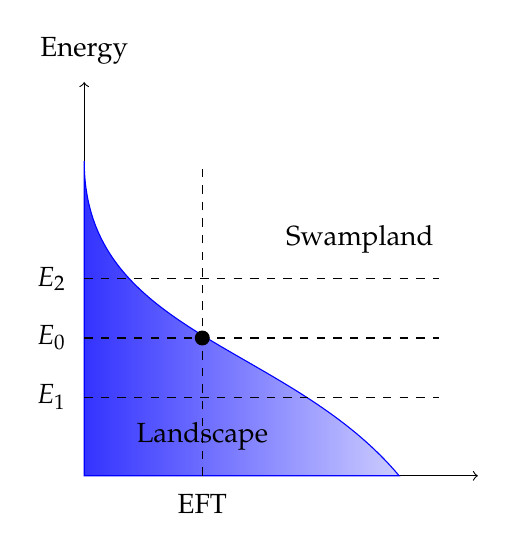
\begin{tikzpicture}[scale = 5]

        \draw[->] (0,0) -- (1,0);
        \draw[->] (0,0) -- (0,1) node[above=3pt]{Energy};
        \shadedraw[left color=blue!80!white,right color=blue!20!white, draw=blue] (0,0) -- (0,0.8) to [out=270, in=130] (0.8,0) -- cycle
        (0,0.2) node[left=3pt]{$E_{1}$}
        (0,0.5) node[left=3pt]{$E_{2}$}
        (0.3,0.1) node{Landscape}
        (0.7,0.6) node{Swampland};
        \draw[style=dashed] (0.3,0) node[below=3pt]{EFT} -- (0.3,0.8);
        \draw[style=dashed] (0,0.35) node[left=3pt]{$E_{0}$} -- (0.9,0.35);
        \draw[style=dashed] (0,0.2) -- (0.9,0.2);
        \draw[style=dashed] (0,0.5) -- (0.9,0.5);
        \filldraw[black](0.3,0.35) circle (0.5pt);
    \end{tikzpicture}
    \caption{This shows the cross section of figure \ref{fig:swampland}. Given an EFT at some lower energy scale, it belongs to the landscape as long as its characteristic energy is below $E_{0}$. However, the same EFT turns to be in the Swampland if the energy scale is above it. For instance, this EFT is in the landscape if it provides a description of physics of energy $E_{1}$, while it is in the Swampland if it does of $E_{2}$.}
    \label{fig:cross}
\end{figure}
Thus, whether an EFT belongs to the Swampland or the landscape is determined by at which energy scale it is used for an illustration of a physical system. As such energy increases, there are more strict constraints, and eventually the landscape gets smaller and smaller.

\subsection{Swampland Conjectures}
Those sonctraints are still investigated and not uderstood well yet. It is why they are called the Swampland conjectures, not being proven yet. However, they have been gradually accepted widely as sufficient amont of evidence to support them has been collected. Figure \ref{fig:connection} shows the conjectures and connections among them.
\begin{figure}
    \centering
    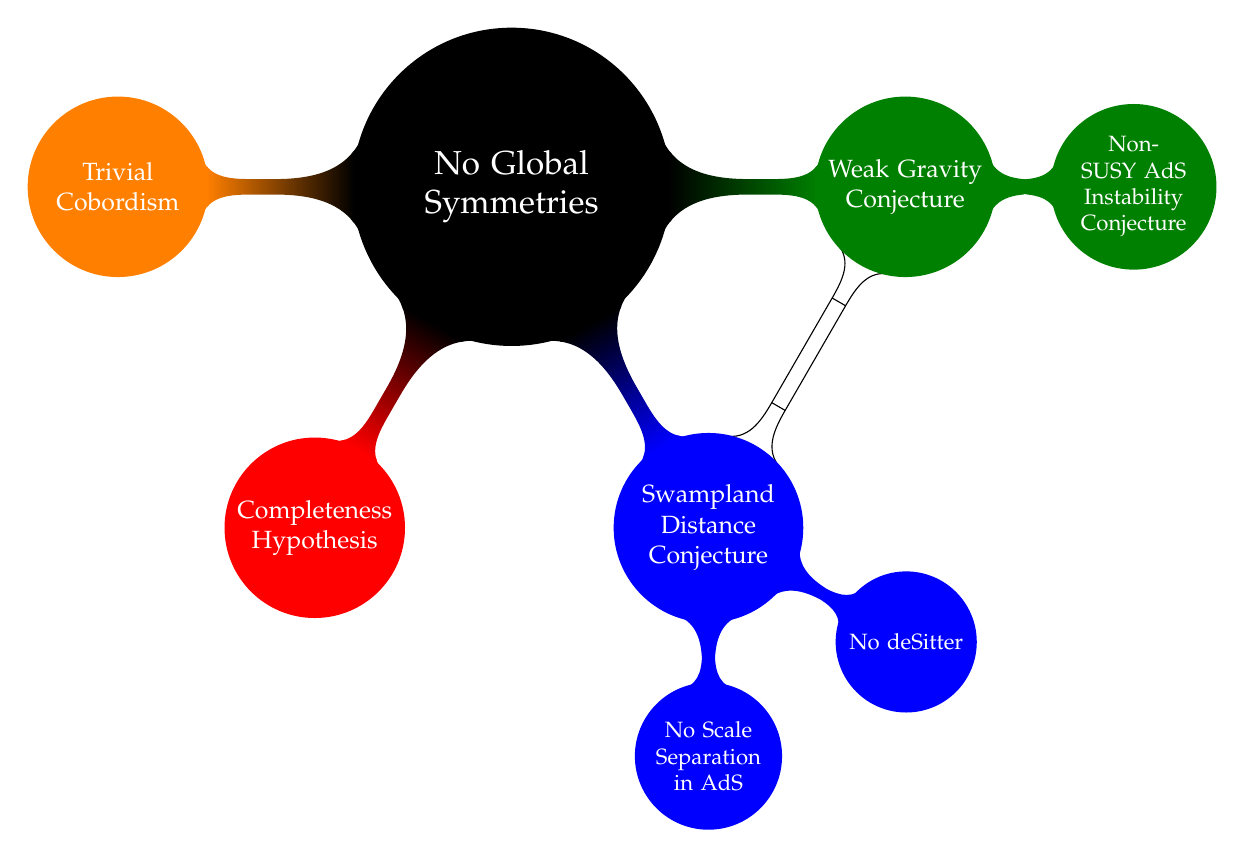
\begin{tikzpicture}
        \path[mindmap,concept color=black,text=white]
    node[concept] {No Global Symmetries}
    [clockwise from=0]
    child[concept color=green!50!black] {%
      node[concept](WG){Weak Gravity Conjecture}
      [clockwise from=0]
      child {node[concept] {Non-SUSY AdS Instability Conjecture} }
      %child {node[concept] {data structures} }
      %child {node[concept] {pro\-gramming languages} }
      %child {node[concept] {software engineer\-ing} }
    }  
    child[concept color=blue] {%
      node[concept](DC) {Swampland Distance Conjecture}
      [clockwise from=-30]
      child {node[concept] {No deSitter} }
      child {node[concept] {No Scale Separation in AdS} }
    }
    child[concept color=red] {node[concept] {Completeness Hypothesis} }
    child[concept color=orange] {node[concept] (TC){Trivial Cobordism} };
    \begin{pgfonlayer}{background}
        \draw [circle connection bar]
        (WG) edge (DC);
    \end{pgfonlayer}
    \end{tikzpicture}
    \caption{A schematic map of the Swampland conjectures}
    \label{fig:connection}
\end{figure}
In the following sections, only two conjectures will be discussed in detail, which are most relevant for the purpose of the thesis. The connestions between conjectures might indicate that some of them are equivalent statements with different appearances. Unifying them by better understanding of QG in the future is one of the goal of this area.

\subsection{No Global Symmetries in Quantum Gravity}
The absence of global symmetries is considered as the first Swampland conjecture, and widely accepted. The statement of the conjecture is as follows:
\begin{tcolorbox}[title=No Global Symmetries Conjecture,
    title filled=false,
    colback=blue!5!white,
    colframe=blue!75!black]
    There are no exact global symtries in quantum gravity.  %\textbf{tcolorbox}.
\end{tcolorbox} 
First of all, it is worth to recall briefly that a global symmetry is defined as an invariance under transformations described by a unitary operator commuting with the Hamiltonian. According to Noether's theorem, the continuous symmetry of a system indicates the existence of the conserved quantity, or charge, in it. For instance, the spatial translational symmetry leads to the conservation of momentum. In order to see illustrate what would make it invalid if a global symmetry is allowed in quantum gravity, assume that there \emph{IS} a continuous global symmetry with a conservation charge in quantum gravity. Suppose a black hole is charged by throwing a conserved charge into it under a $U(1)$ global symmetry, it will evaporate decreasing its mass but maintaining its charge because Hawking radiation contains same number of positive/negative charged particles. Letting it evaporate completely, charge is supposed to vanish. Thus, it leads to a violation of the charge conservation. Also, even if such evaporation stops , and ends up with a remnant of mass $M \sim M_{P}$, since, according to the No-hair theorem, stable black holes can be distinguished from outside only by its mass, angular momentum, and gauge charge, it is impossible to determine its global charge given a black hole of a specific mass. Therefore, the conservation gets invalid. Hence, there cannot be global symmetries in a theory of quantum gravity.This discussion can be extended to discrete symmetries and also to more generic global symmetries. Those are followed by the proposal of the Cobordism conjecture, which will be presented later. The arguments above are rather motivation that proofs to grasp good intuitions for the conjecture. There are more formal evidences mainly from string theory. Here most of discussions for such proofs is from %\parencite{}.
It is important to note that it is permitted that there is a low-energy theory with a global symmetry, as long as at higher energies such symmetry is gauged or broken. While it still gives understanding of the principles of quantum gravity, the No-global symmetries conjecture doesn't provide meaningful phenomenological constraints since nothing about at which scale such a global symmetry gets forbidden is stated. However, it is followed by other conjectures such as the Weak Gravity Conjectures and the Swampland Distance Conjecture, which give more concrete constraints, as expansions and refinements of the concept of the impossibility of exact global symmetries in quantum gravity. 
\subsection{Swampland Distance Conjecture}
The Swampland Distance Conjecture (SDC) is the one of the Swampland conjectures which give certain quantitative constraints. It provides a restriction on an EFT of quantum gravity when it is getting closer to where a global symmetry is restored. \\
\indent The motivation for the conjecture comes from the investigation in a moduli space, which is a space parametrized by the vacuum expectation value of some scalar fields. It is particular interest in that space to observe how an EFT changes as moving toward a certain direction where a global symmetry gradually, that is, some gauge coupling decreases to zero, because an exact global symmetry is not acceptable in quantum gravity. Therefore it is expected there is some phenomena in such limits in order to protect a theory to get back a global symmetry. One natural assumption to do so is that such poins are infinitely far away in a space. In addition, as an approximate global symmetry is getting exact as moving towards those limits, it is reasonable that an EFT is supposed to become an invalid description continuously. That is also predicted by the consequence of the Weak Gravity Conjecture. \\
\indent One important key point is that it is characteristic for a quantum gravity. Without considerring the quantum gravity, it is perfectly fine to have a point where a gauge coupling vanishes at infinite distance, and being close to it with maintaining a valid theory. Once the quantum gravity is taken into account, since taking a exact global symmetry strictly forbidden, an EFT should break down continuously as being closing to those limits. This can be generalized to other types of global symmetries. The Swampland Distance Conjecture provides information how EFT behaves when approaching infinite distance in a moduli space, and what features of quantum gravity makes it happen. \\
\indent Consider an EFT coupled to Einstein gravity with moduli space $\mathcal{M}$ parametrized by scalar fields, and whose metric $g_{ij}$ is given by its kintic term. The first statement of the conjecture is as follows: Starting from a point $P \in \mathcal{M}$, there always exits a point $Q \in \mathcal{M}$ at infinite geodesic distance $d(P,Q)$. The second part of the conjecture describes a phenomena supposed to happen as approaching a point at infinite field distance:
\begin{tcolorbox}[title=Swampland Distance Conjecture,
    title filled=false,
    colback=blue!5!white,
    colframe=blue!75!black]
    There happens an infinite tower of states which becomes exponentially light with the geodesic distance such as 
    \begin{align}
        M(Q) \sim M(P) e^{-\lambda d(P,Q)}
    \end{align}
    with $\lambda$ an $\order*{1}$ constant in Planck units. 
\end{tcolorbox}
It is abstractly illustrated in figure \ref{fig:tower}. Since an EFT cannot deal with infinitely many degrees of freedom under its cut-off, the emergence of the infinite tower of states indicates the breakdown of EFT. Thus, there supposed to be a quantum gravity cut-off associated to the infinite tower of states, which decreases exponentially with the geodesic distance:
\begin{align}
    \Lambda _{\text{QG}} = \Lambda e^{-\lambda d(P,Q)}
\end{align}
\begin{figure}
    %\centering
    \begin{subfigure}{.5\linewidth}
        %\centering
        \begin{tikzpicture}[scale=5]
            \draw[->] (0,0) -- (0,1) node[above=3pt]{M};
            \draw[style = dashed] (-0.4,0.8) node[left=3pt] {$\Lambda$} -- (0.4,0.8);
            \draw[-] (-0.03,0.1) -- (0.03,0.1);
            \draw[-] (-0.03,0.2) -- (0.03,0.2);
            \draw[-] (-0.03,0.3) -- (0.03,0.3);
            \draw[-] (-0.03,0.4) -- (0.03,0.4);
            \draw[-] (-0.03,0.5) -- (0.03,0.5);
            \draw[-] (-0.03,0.6) -- (0.03,0.6);
            \draw[-] (-0.03,0.7) -- (0.03,0.7);
            \draw[-] (-0.03,0.9) -- (0.03,0.9);
        \end{tikzpicture}
    \end{subfigure}
    \begin{subfigure}{.5\linewidth}
        %\centering
        \begin{tikzpicture}[scale=5]
            \draw[->] (0,0) -- (0,1) node[above=3pt]{M};
            \draw[style = dashed] (-0.4,0.8) node[left=3pt] {$\Lambda$} -- (0.4,0.8);
            \draw[-] (-0.03,0.1) -- (0.03,0.1);
            \draw[-] (-0.03,0.2) -- (0.03,0.2);
            \draw[-] (-0.03,0.3) -- (0.03,0.3);
            \draw[-] (-0.03,0.4) -- (0.03,0.4);
            \draw[-] (-0.03,0.5) -- (0.03,0.5);
            \draw[-] (-0.03,0.6) -- (0.03,0.6);
            \draw[-] (-0.03,0.7) -- (0.03,0.7);
            \draw[-] (-0.03,0.9) -- (0.03,0.9);
            \draw[-] (-0.03,0.65) -- (0.03,0.65);
            \draw[-] (-0.03,0.75) -- (0.03,0.75);
            \draw[-] (-0.03,0.55) -- (0.03,0.55);
            \draw[-] (-0.03,0.45) -- (0.03,0.45);
            \draw[-] (-0.03,0.35) -- (0.03,0.35);
            \draw[-] (-0.03,0.25) -- (0.03,0.25);
            \draw[-] (-0.03,0.15) -- (0.03,0.15);
            \draw[-] (-0.03,0.05) -- (0.03,0.05);
        \end{tikzpicture}
    \end{subfigure}
    \caption{Left picture represents an EFT with a cut-off $\Lambda$. There are finitely many states below this cut-off. As moving toward a point at infinite geodesic distance, it becomes as shown right. Continuously, the closer it is to such a point, the more degrees of freedom coming in the EFT description. After all, in order to try to avoid infinitely many degrees of freedom for an EFT, a cut-off is supposed to fall down to zero.}
    \label{fig:tower}
\end{figure}
\indent To gain an insight how SDC is realized, consider an example of a theory compactified on a circle of radius R. Through a Kaluza-Klein circle compactification in such a circle, its modes, KK modes, are known to have a mass as:
\begin{align}
    \label{eq:1.3}
    m_{n}^{2} = \frac{n^{2}}{R^{2}} ,& \qq{} n \in \mathbb{Z}. 
\end{align}
Taking this R to be the modulus controlling the radius of the circle, the kinetic term of the field R can be written in $\mathcal{L} _\text{{kin}} \sim \frac{1}{R^{2}} \partial_{M} R \partial ^{M} R$. The geodesic distance between two points, namely $R_{i}$ and $R_{f}$, in the field space is mesured by the metric, and yields to:
\begin{align}
    d(R_{i},R_{j}) = \abs \Big{\ln (R_{f} / R_{i})}
\end{align} 
From this, it is easy to see that there are two points which give an infinite proper distance starting from any finite radius, $R \to \infty$ and $R \to 0 $. The first limit gives a predicted behavior from eq. \ref{eq:1.3}. On the contrary, it seems that the SDC is violated for the limit $R \to 0$. However, considering the string theory, which has another infinite tower of states, winding states, whose masses given:
\begin{align}
    \label{eq:1.5}
    m_{w} ^2 = \frac{w^{2} R^{2}}{(\alpha ')^2}
\end{align}
where $\alpha '$ stands for the string length, and they also behave as expected. In this sense, there is a critical connection betweem the realization of SDC and the existence of T-duality. \\
\indent To sum up, the SDC can be thought of as a constraint on the validity for finite field variations, as an EFT at a point in moduli space cannot be extended to an arbitrary far point from initial one. By approaching such a point, an infinite number of degrees of freedom would become exponentially light and eventually an EFT description broken. So far computations for the distance ahve been considered on the moduli space. Nevertheless, this notion of the distance can be generalized to the one between more generic field with a generic metric given also by the kinetic term. It will be investigated how the renoemalization group affects on the statement of this conjecture later. 
\subsection{Other Conjectures}

\chapter{Renormalization Group}
\label{RG}
Since it is central for this thesis to see how the renormalization group (RG) affects on the SDC, another preliminary we need before the computaion is the concept of renormalization group and how we can carry out the calculations. In this chapter, first we will have introductions to the renormalization group (RG) starting from a review of the generating functional to the beta function, or the RG equations. Understanding the basics of RG, we will provide a specific method for our later computation, named Heat Kernel expansion.

\section{Focused Review of Generating Functional}
Consider a theory with n fields $\phi^{i} (x)$, $i = 1, \dotso , n$, governed by a classical action $S[\phi]$, and suppose computing its correlation functions:
\begin{align}
    G^{i_{1}, \dotso , i_{n}} (x_{1}, \dotso ,x_{n} ) := \mel{\Omega _{f}}{T[\phi^{i_{1}}(x_{1}) \dots \phi^{i_{n}} (x_{n})]}{\Omega _{i}}
\end{align}
where $\ket{\Omega}$ stands for the ground state in the past or future, and T indicates time ordering. We can extract general observables of the system such as scattering amplitudes from them. By introducing the generating functional $Z[J]$, we can deal with such correlators at onece. Definition of $Z[J]$ is:
\begin{align}
    Z[J] := \sum_{n=0} ^{\infty} \frac{i^{n}}{n!} \int d^{4}x_{1} \dotso d^{4}x_{n}   G^{i_{1}, \dotso , i_{n}} (x_{1}, \dotso ,x_{n} ) J_{i_{1}}(x_{1}) \dots J_{{i_{n}}}(x_{n})
\end{align}
then each correlation function can be in a form by functional differentiation:
\begin{align}
    G^{i_{1}, \dotso , i_{n}} (x_{1}, \dotso ,x_{n} ) = (-i)^{n} (\frac{\delta^{n}Z[J]}{\delta J_{i_{1}}(x_{1}) \dots \delta J_{i_n} (x_{n})}) _{J=0}
\end{align}
The generating functional is useful because it is a simple expression in terms of path integral formalism. Such simplicity means not only the easiness to be computed but also practically that it is relatively straightforward to compute perturbatively in terms of Feynman diagrams. 
\begin{align}
    G^{i_{1}, \dotso , i_{n}} (x_{1}, \dotso ,x_{n} ) = \int \mathcal{D} \phi e^{iS[\phi]} \phi^{i_1} (x_{1}) \dots \phi ^{i_{n}}(x_n)
\end{align}
where the integration measure is:
\begin{align}
    \int \mathcal{D} \phi = \prod_{x^{\mu}} \int d\phi(x)
\end{align}
The special case $n=0$ is the typical example for which
\begin{align}
    \braket{\Omega _{f}}{\Omega _{i}} = \int \mathcal{D} \phi e^{iS[\phi]}
\end{align}
Using the definition, we can obtain the following expression for the generating functional:
\begin{align}
    Z[J] = \int \mathcal{D} \phi exp\lbrace iS[\phi] + i \int d^{4}x \phi^{i} (x) J_{i} (x) \rbrace
\end{align}
and immediately find:
\begin{align}
    Z[J=0] = \braket{\Omega _{f}}{\Omega _{i}}
\end{align}

\subsubsection{Semiclassical Evaluation}
Expand the action about a classical background so that:
\begin{align}
    \phi(x) = \varphi_{\text{cl}} (x) + \tilde{\phi}(x) 
\end{align}
where $\varphi_{\text{cl}}$ fulfills:
\begin{align}
    \label{eq:semi}
    \eval {\fdv{S}{\phi}}_{\phi = \varphi_{\text{cl}}} + J = 0
\end{align}
Suppose we have an action $S_{j}[\phi] := S[\phi] + \int d^{4}x (\phi ^{i} J_{i})$, and want to write it in a form:
\begin{align}
    S_{j} [\varphi_{\text{cl}} + \tilde{\phi}] = S_{J}[\varphi _{\text{cl}}] + S_{2} [\varphi _{\text{cl}}, \tilde{\phi}] + S_{\text{int}}[\varphi_{\text{cl}}, \tilde{\phi}]
\end{align} 
where:
\begin{align}
    S_{2} = -\int d^{4} x \tilde{\phi^{i}}\Delta _{ij}(\varphi_{\text{cl}}) \tilde{\phi ^{j}}
\end{align}
being the quadratic part in the expansion for some differential operator $\Delta _{ij}$. $S_{\text{int}}$, namely interaction term, contains higher order terms in $\tilde{\phi^{i}}$. Notice that since the background field satisfies eq.\ref{eq:semi}, there will be no linear terms. \\
\indent Then the expression inside the above path integral can be expanded as:
\begin{align}
    \exp \lbrace iS[\phi] + i\int d^{4}x \phi^{i}J_{i} \rbrace = \exp \lbrace iS_{J}[\varphi_{\text{cl}}]+ iS_{2} [\varphi_{\text{cl}}, \tilde{\phi}] \rbrace \sum_{r=0}^{\infty} \frac{1}{r!} (iS_{\text{int}}[\varphi_{\text{cl}},\tilde{\phi}])^{r}
\end{align}
This will be followed by the graphical representation of any correlators. Gaussian integrals involve integrands which are powers of fields:
\begin{align}
    \int \mathcal{D} \tilde{\phi} e^{i\tilde{\phi}^{i}\Delta _{ij} \tilde{\phi}^{j}} \tilde{\phi}^{k_{1}}(x_{1}) \dots \tilde{\phi}^{k_{n}} (x_{n}) \propto (\text{det}^{-1/2} \Delta) [(\Delta ^{-1})^{k_{1}k_{2}} \dots (\Delta ^{-1})^{k_{n-1}k_{n}} + (\text{permutations})]
\end{align}
for even $n$, while the integrand vanishes if $n$ is odd. The combinatorics in an integral correspond to the combinatorics of all posiible ways to connect graphs whose internal lines represent factors of $\Delta ^{-1}$ and vertices to interactions within $S_{\text{int}}$. In this language, $Z[J]$ denotes the sum over all vacuum graphs with no external lines. Some leading perturbative contributions to the generating functional are:
\begin{align}
    Z[J] = N (\text{det}^{-1/2} \Delta)[ 1+
    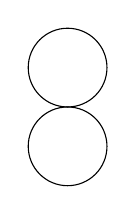
\begin{tikzpicture}
        \draw (0,0) circle (0.5);
        \draw (0,-1) circle (0.5);
    \end{tikzpicture}
    ]
\end{align}
where solid lines are propagators and black dots represent interactions appear in $S_{\text{int}}$. \\ This indeed includes all graphs containing those that are disconnected. Such graphs are disconnected in the sense that it is not possible to get between any pair of vertices along some sequence of internal lines. \\
\indent Those expansions here are not practical yet in order to carry out the explicit computaions because of the appearance of the background field in the propagator $\Delta _{ij}(x,y) = \frac{\delta^{2}S}{\delta \phi ^{i}(x) \delta \phi ^{j}(y)}$. For example, for a scalar field wit a scalar potential $U(\phi)$, we have $\Delta(x,y) = [-\square + U'' (\varphi)]\delta ^{4} (x-y)$. This is easily inverted in momentum space if $\varphi$ is constant, but is not straightforward to invert for arbitrary $\varphi(x)$. Such a problem is often addressed by expanding in powers of $J_{i}(x)$ so that path integral is evaluated as a semiclassical expansion about a simple backgroud configuration $\varphi _{\text{cl}}^{i}$ which satisfies:
\begin{align}
    \eval{\fdv{S}{\phi ^{i}}}_{\phi = \varphi _{\text{cl}}} = 0
\end{align}
By doing this, for the modified expansion the term $\phi^{i} J_{i}$ in the exponent of the integrand is viewed as an interaction. This is linear in $\phi ^{i}$, so it corresponds to a tadpole contribution, with the line ending in a cross whose Feynman rule is $J_{i}(x)$.

\subsection{Connected Correlation}
Instead of dealing with all graphs including both connected and disconnected, it is usually useful to work with a generating functional $W[J]$ whose graphical representaion contains only connected ones. This is achieved by defining as $Z[J] := \exp \lbrace iW[J] \rbrace$, because taking logarithm means subtracting the disconnected graphs. This leads:
\begin{align}
    \label{eq:W}
    \exp \lbrace iW[J] \rbrace = \int \mathcal{D} \phi \exp \lbrace iS[\phi] + i\int d^{4}x \phi ^{i} J_{i} \rbrace 
\end{align}
Then corresponding correlation functions are given:
\begin{align}
    \expval{T[\phi ^{i_{1}}(x_{1}) \dots \phi ^{i_{n}}(x_{n}) ]} := (-i)^{n-1} \eval{\frac{\delta ^{n}W[J]}{\delta J_{i_{1}}(x_{1}) \dots \delta J_{i_{n}}(x_{n})}} _{J=0}
\end{align}

\subsection{The 1-Particle Irreducible Action}
As discussed, $Z[J] = \exp \lbrace iW[J] \rbrace$ can be thought of as the 'in-out' vacuum amplitude with a current $J_{i}$. In addition, the current can be interpreted as being responsible for varying the expectation value of the field since at $J_{i}  = 0$:
\begin{align}
    \varphi^{i} (x) := \expval{\phi^{i}(x)} = \fdv{W}{J_{i} (x)}
\end{align}
But it is often more simple to have the vacuum-to-vacuum amplitude expressed as in terms of a functional of the expectation value $\varphi ^{i}$. This can be done through a Legendre transform. In order to perform Legendre transform, we may define:
\begin{align}
    \Gamma [\varphi] := W[J] - \int d^{4}x \varphi ^{i}J_{i}
\end{align}
here $J_{i}(x)$ is a functional of $\varphi ^{i}(x)$. Then we have a relation:
\begin{align}
    \fdv{\Gamma}{\varphi^{i}(x)} = -J_{i}(x)
\end{align}
It shows that the expectation value for the system with $J_{i}=0$ is a stationary point of $\Gamma[\varphi]$. Therefore, the relation between $\Gamma[\varphi]$ and $\expval{\phi^{i}}$ is to the one between the classical action and a classical background configuration. 
\subsubsection{Semiclassical Expansion}
Now consider about the computation of $\Gamma[\varphi]$ within perturbation theory. From eq.\ref{eq:W}, we may have:
\begin{align}
    \begin{split}
        \exp \lbrace i\Gamma[\varphi]\rbrace &= \exp \lbrace iW[J] - i\int d^{4}x \varphi^{i} J_{i} \rbrace \\
        &= \int \mathcal{D} \phi \exp \lbrace iS[\phi] + i \int d^{4}x (\phi ^{i} - \varphi ^{i})J_{i} \rbrace \\
        &= \int \mathcal{D} \tilde{\phi} \exp \lbrace iS[\varphi + \tilde{\phi}]+ i\int d^{4}x \tilde{\phi} ^{i} J_{i}
    \end{split}
\end{align}
in the last line we changed the integration variable as $\phi ^{i} \rightarrow \tilde{\phi}^{i} := \phi ^{i} - \varphi ^{i}$. Expanding the action inside the path integral about $\phi^{i} = \varphi ^{i}$:
\begin{align}
    S[\varphi + \tilde{\phi}] = S[\varphi] + S_{2} [\varphi, \tilde{\phi}] + S_{\text{int}}[\varphi,\tilde{\phi}]
\end{align}
This is a similar expression we had before except the term linear in $\tilde{\phi}^{i}$:
\begin{align}
    S_{\text{int}}[\varphi,\tilde{\phi}] = \int d^{4}x [\eval{\fdv{S}{\phi^{i}}(x)}_{\phi=\varphi} + J_{i}(x)] \tilde{\phi}^{i}(x)
\end{align}
which does not vanish since $\delta \varphi^{i} := \varphi ^{i} - \varphi_{\text{cl}}^{i} \neq 0$. However, $\delta\varphi^{i}$ is perturbatively so small that it would be within $S_{\text{int}}$, expanded within the integrand, and not kept in the exponential. The expantion eventually becomes:
\begin{align}
    e^{i\Gamma[\varphi]} = e^{iS[\varphi]} \int \mathcal{D}\tilde{\phi} e^{iS_{2}[\varphi,\tilde{\phi}]}\sum _{r=0}^{\infty} \frac{1}{r!}(iS_{\text{int}}+ i S_{\text{lin}})^{r}
\end{align}
and then:
\begin{align}
    \label{eq:Gamma}
    \Gamma[\varphi] = S[\varphi] + \frac{i}{2}\ln \det \Delta + (\text{more than 1-loops})
\end{align}
The first two terms in eq.\ref{eq:Gamma} are the classical and one-loop contributions respectively, though the last contains the sum over all Feynman graphs with two or more loops. \\
\indent Since $S_{\text{lin}}$ is linear term in $\tilde{\phi}^{i}$, its Feynman rule is as seen before, which inserts a tadpole contribution proportional to $\fdv{S}{\varphi ^{i}} + J_{i}$. Notice that evaluationg at $J_{i} = -\fdv{\Gamma}{\varphi ^{i}}$, eq.\ref{eq:Gamma} gives:
\begin{align}
    \begin{split}
    \fdv{S}{\varphi^{i}(x)} + J_{i}(x) &= \fdv{\varphi^{i}(x)} (S[\varphi] - \Gamma[\varphi])\\
    &= - \fdv{\varphi^{i}(x)} [\frac{i}{2} \ln \det \Delta + (\text{more than 1-loops})] \\
    & = -(\text{sum of tadpole graphs})
    \end{split}
\end{align}
Therefore, we can manipulate without knowing expression for $\Gamma[\varphi]$. $J_{i} =-\fdv{\Gamma}{\varphi}$ imdicates that all graphs involving explicit dependence on $J_{i}$ cancel all graphs which can be split into two disconnected graphs. In this language, a graph which cannot be separated into tow pieces is called 1-particle irreducible (1PI). Thus, $\Gamma[\varphi]$ can be obtained by evaluating only 1PI graphs. Therefore, $\Gamma[\varphi]$ is often called the generator of 1PI correlations, or 1PI action. In semiclassical expansion, eq.\ref{eq:Gamma} is computed as a sum of 1PI connected graphs without external lines. \\
\indent Viewing $\Gamma[\varphi]$ only involves 1PI suggests alternative way in which $\Gamma[\varphi]$ generalizes the classical action. In a perturbative expansion the leading approximation is the leading term in $\Gamma[\varphi] \approx S[\varphi]$. Considering scattering amplitudes, this amounts to summing the tree level graphs from vertices from the classical interactions in $S_{\text{int}}$. On the other hand, suppose computing Feynman graphs by the expansion of $\Gamma[\varphi + \tilde{\phi}]$ to obtain the propagators and vertices. For this, loops for any correlators with Feynman rules for $S[\varphi]$ is same as the quantities given by summing all tree graphs made from the Feynman rules for $\Gamma[\varphi]$. Thus, the full quantum amplitude can be found by computing with $\Gamma[\varphi]$ within the classical approxiamtion. 

\section{Wilsonian Effective Action}
Now let us consider a field theory with characteristic (large) energy scale $M$, and suppose we want to study physics at a lower energy regime namely $E \ll M$. This is precisely the situation the EFTs are useful. The full theory is defined in terms of the path integral, and we can extract observables from calculating the correlator:
\begin{align}
    \mel{0}{T[\phi(x_{1}) \dotso \phi(x_{n})]}{0} = \frac{1}{Z}\int \mathcal{D} \phi e^{iS[\phi]} \phi(x_{1}) \dots \phi(x_{n})
\end{align}
with the integration measure is:
\begin{align}
    \int \mathcal{D}\phi = \prod_{x^{\mu}} \int d\phi(x)
\end{align}
and
\begin{align}
    Z = \int \mathcal{D}\phi e^{iS[\phi]}
\end{align}
Then consider what happend as we try to perform the path integral by integrating those modes first with energy between $\Lambda _{0}$ and $\Lambda < \Lambda_{0}$. We can split a generic field $\phi(x)$ as:
\begin{align}
    \begin{split}
        \phi(x) &= \int _{\abs{p} \le \Lambda_{0}} \frac{d^{d}p}{(2\pi)^{d}} e^{ip\dot x} \tilde{\phi}(p) \\
        &= \int _{\abs{p} \le \Lambda} \frac{d^{d}p}{(2\pi)^{d}} e^{ip\cdot x} \tilde{\phi}(p) + \int _{\Lambda < \abs{p} \le \Lambda _{0}} \frac{d^{d}p}{(2\pi)^{d}} e^{ip\cdot x} \tilde{\phi}(p) \\
        & := \varphi (x) + \chi (x)
    \end{split}
\end{align}
where $\varphi(x)$ and $\chi(x)$ are low- and high-energy part of the field respectively. Thus the path integral measure can be rewritten as:
\begin{align}
    \mathcal{D}\phi = \mathcal{D} \varphi \mathcal{D} \chi
\end{align}
into a product of measures over low- and high-energy modes. Since we are now interested in low-energy physics, we just need to compute the correlation function:
\begin{align}
    \mel{0}{T[\varphi(x_{1}) \dotso \varphi(x_{n})]}{0} = \frac{1}{Z} \int \mathcal{D} \varphi \int \mathcal{D} \chi e^{iS[\varphi + \chi]} \varphi(x_{1}) \dotso \varphi(x_{n})
\end{align}
Then we define a Wilsonian effective action at scale $\Lambda$ $S_{\Lambda}[\varphi]$ as follows:
\begin{align}
    e^{iS_{\Lambda}[\varphi]} := \int \mathcal{D}\chi e^{iS[\varphi + \chi]}
\end{align}
and we have chosen $\Lambda < M$ to integrate out the physics associated with $M$. $S_{\Lambda} [\varphi]$ is non-local n scales $\Delta x^{\mu} \gtrsim \frac{1}{\Lambda}$, that is, the Lagrangian is not just a polynomial of the fields or their derivatives evaluated at a single point in spacetime, since high-energy fluctuations have been integrated out. Expanding the non-local action a series of local operators:
\begin{align}
    S_{\Lambda} [\varphi] &= \int d^{d}x \mathcal{L}_{\Lambda}^{\text{eff}}(x) \\
    \mathcal{L}_{\Lambda}^{\text{eff}(x)} &= \sum_{i} g_{i}\mathcal{O}_{i}(x)
\end{align}
here $\mathcal{L}_{\Lambda}^{\text{eff}}(x)$ is an effective Lagrangian at scale $\Lambda$.  It is an infinite sum over local operators $\mathcal{O}_{i}$ allowed by symmetries. The coefficients gi are referred to as Wilson coefficients.
\subsection{Running Couplings and Their Beta-functions}
It is important to notice that the partition function:
\begin{align}
    Z_{\Lambda} (g_{i} (\Lambda)) = \int _{\le \Lambda} \mathcal{D} \phi e^{-iS_{\Lambda}[\phi]}
\end{align}
obtained from the effective action at scale $\Lambda$ is exactly the same as the one we started with:
\begin{align}
    Z_{\Lambda}(g_{i}(\Lambda)) = Z_{\Lambda_{0}}(g_{i0};\Lambda_{0})
\end{align}
because we are just computing the remaining integrals over the low-energy modes. Particularly, as the scale is lowered infinitesimally, this becomes:
\begin{align}
    \label{eq:rgpf}
    \Lambda\dv{Z_{\Lambda}(g)}{\Lambda} = (\eval{\Lambda \pdv{\Lambda}}_{g_{i}} + \Lambda\pdv{g_{i}(\Lambda)}{\Lambda} \eval{\pdv{g_{i}}}_{\Lambda})Z_{\Lambda}(g) = 0
\end{align}
Eq.\ref{eq:rgpf} is known as the renormalization group equation for the partition function. It is claiming that as we change the scale by integrating out modes, the couplings in the effective action $S_{\Lambda}$ vary to account for the change in the degrees of freedom over which we take the path integral so that the partition function is indeed independent of the scale at which we define our theory, provided this scale is below our initial cut-off scale $\Lambda_{0}$. Since the running of couplings is so important, it has a specific name and we can define the beta-function $\beta _{i}$ of the coupling $g_{i}$ to be the derivative with respective to the logarithm of the scale:
\begin{align}
    \beta_{i} := \Lambda\pdv{g_{i}}{\Lambda} = \pdv{g_{i}}{\ln \Lambda}
\end{align}


\subsection{1PI for Wilsonian Action}
Here let us consider the 1PI for a Wilsonian effective action $S_{\Lambda} [\varphi]$ following the procedure in previous section. To begin with, for our convinience by the Wick rotation we may have:
\begin{align}
    S_{\Lambda}[\varphi] := iS_{E,\Lambda}[\varphi]
\end{align}
and from now on we will just write this as $S_{\Lambda}[\varphi]$ unless it makes serious confusions. Then the generating functional for the Green functions of a field $\varphi$ in the path integral representaion is:
\begin{align}
    \begin{split}
        Z[J] &= \int \mathcal{D}\varphi \exp (-S_{\Lambda} [\varphi] - \int d^{d}x J(x)\varphi(x)) \\
        & = \int \mathcal{D} \varphi \exp (-\int d^{d}x (\mathcal{L} [\varphi(x)] + J(x)\varphi(x)))
    \end{split}
\end{align}
with an external source $J(x)$. Suppose then that a field $\varphi (x)$ can be splitted into two pieces: a classical background $\zeta(x)$ and a quantum fluctuations $\eta (x)$ so that:
\begin{align}
    \varphi(x) = \zeta(x) + \eta(x)
\end{align}  
with a condition $\eval{\fdv{S}{\varphi}} _{\varphi = \zeta} + J(x) = 0$ is satisfied. Then the expansion of the action around the backgroud gives:
\begin{align}
    \label{eq:expand}
    \begin{split}
    \int d^{d} x  (\mathcal{L}[\varphi(x)] + J(x) \varphi(x) ) = & \int d^{d}x  (\mathcal{L}[\zeta(x)] + J(x)\zeta(x))  \\
    + & \int d^{d} x (\eval{\fdv{\mathcal{L}}{\varphi}} _{\phi = \eta} + J(x)) \eta(x) \\
    + & \frac{1}{2} \int d^{d}x d^{d}y \eval {\frac{\delta ^{2} \mathcal{L}}{\delta \varphi(x) \delta \varphi(y)}} _{\varphi = \zeta} \eta(x)\eta(y) \cdots 
    \end{split}
\end{align}
The second term of eq.\ref{eq:expand} is identically zero due to the equation of motion. Then the generating functional can be in the form:
\begin{align}
    Z[J] = e^ {\qty (-\int d^{d}x (\mathcal {L} [\zeta (x)] + J(x) \zeta (x)))} \int \mathcal {D} \eta e^{- \frac{1}{2} \int d^{d}x d^{d}y \eval {\frac{\delta ^{2} \mathcal{L}}{\delta \varphi(x) \delta \varphi(y)}} _{\phi = \zeta} \eta(x)\eta(y) \cdots}
\end{align}
because the first integral in eq.\ref{eq:expand} has nothing to do with the fluctuation $\eta(x)$. Notice that the remaining path integral over $\eta$ is of Gaussian form and can be computed explicitly:
\begin{align}
    Z[J] = e^ {\qty (-\int d^{d}x (\mathcal {L} [\zeta (x)] + J(x) \zeta (x)))} \qty (\text{det} \frac{\delta ^{2} \mathcal{L}}{\delta \varphi(x) \delta \varphi(y)})^{-1/2} + \cdots
\end{align}
A generating functional $Z[J]$ takes the form $Z[J] = e^{-W[J]}$, then, with an identity $\text{det} \mathcal{A} = e^{\text{Tr} \ln \mathcal{A}}$:
\begin{align}
    W[J] = \int d^{d}x (\mathcal {L} [\zeta (x)] + J(x) \zeta (x)) + \frac{1}{2} \text{Tr} \ln \frac{\delta ^{2} \mathcal{L}}{\delta \varphi(x) \delta \varphi(y)} + \cdots
\end{align}
Performing a Legendre transformation in order to compute the effective action $\Gamma[\varphi]$:
\begin{align}
    \Gamma[\zeta] &= W[J] - \int d^{d} x J(x)\zeta(x) \nonumber \\
    & = \int d^{d}x \mathcal{L} [\zeta(x)] + \frac{1}{2} \text{Tr} \qty[\ln \frac{\delta ^{2} \mathcal{L}}{\delta \varphi(x) \delta \varphi(y)}] + \cdots
\end{align}
The first term is apparently the classical action. Thus the one-loop effective action is given:
\begin{align}
    \label{eq:2.8}
    \Gamma_{\text{1-loop}} [\varphi] = \frac{1}{2} \text{Tr} \qty[\ln \frac{\delta ^{2} \mathcal{L}}{\delta \varphi(x) \delta \varphi(y)}]
\end{align}
The divergent part of eq.\ref{eq:2.8} is the same as the counter-terms, i.e. the action at a renormalized scale. Therefore, it is necessary to be able to carry out this trace in some ways in order to find the beta functions. Here we will adopt the method of Heat Kernel expansion. 

\section{Heat Kernel Expansion}
\subsection{General Formalism}
For the manipulation of the trace, introduce the heat kernel:
\begin{align}
    K(t;x,y;D) = \mel{x}{e^{-tD}}{y}
\end{align}
such that it satisfies the heat conduction equation:
\begin{align}
    (\partial _{t} + D_{x})K(t;x,y;D) = 0
\end{align}
with an initial condition:
\begin{align}
    K(0;x,y;D) = \delta (x-y)
\end{align}
For instance, for a kernel for $ D = - \Delta$:
\begin{align}
    K(t;x,y;-\Delta) = (4\pi t)^{-d/2} \text{exp} ^{\qty (-\frac{(x-y)^2}{4t})}
\end{align}
and for $D = D_{0}= -\Delta +m^2 $:
\begin{align}
    K(t;x,y;D) = (4\pi t)^{-d/2} \text{exp}^{ \qty (-\frac{(x-y)^2}{4t} - tm^2)}
\end{align}
For a general D, $K(t;x,y;D_{0})$ still describes the leading singularity at $t \to 0$:
\begin{align}
    K(t;x,y;D) = K(t;x,y;D_{0}) (1 + tb_{2} (x,y) + t^{2} b_{4}(x,y) + \cdots)
\end{align}
Coefficients $b_{k} (x,y)$ are regular in the limit $y \to x$, and called the heat kernel coefficients. \\
\indent It is needed to compute the functional:
\begin{align}
    \Gamma_{\text{1-loop}} = \frac{1}{2} \Tr \ln D
\end{align}
where;
\begin{align}
    D = \frac{\delta^2 \mathcal{L}}{\delta \phi \delta \phi} 
\end{align}
But for each positive eignevalue $\lambda$ of the operator $D$, an identity is:
\begin{align}
    \ln \lambda = -\int _{0} ^{\infty} \frac{dt}{t} e^{-t\lambda}
\end{align}
Then eq.\ref{eq:2.8} can be rewritten:
\begin{align}
    \Gamma _{\text{1-loop}} = -\frac{1}{2} \int _{0}^{\infty} \frac{dt}{t} K(t,D)
\end{align}
where 
\begin{align}
    K(t,D) = \Tr e^{-tD} = \int d^{d} x \sqrt{g} K(t;x,x;D)
\end{align}
To see a UV divergence, introduce a cut-off at $t=\Lambda ^{-2}$, and compute a part of $\Gamma _{\text{1-loop}}$ which diverges in the limit $\Lambda \to 0$:
\begin{align}
    \begin{split}
    \Gamma _{\text{1-loop}} ^{\text{div}} =&  -(4\pi)^{-d/2} \int d^{d} x \sqrt{g} [ \sum_{2(j+l)< d} \Lambda ^{d-2j-2l} b_{2j}(x,x) \frac{(-m^{2})^{l} l!} {d-2j-2l}  \\
    &+ \sum_{2(j+l) =d} \ln \Lambda (-m^{2})^{l} l! b_{2j} (x,x) + \order {\Lambda ^{0}} ] 
    \end{split}
\end{align}
It can be seen that the UV divergence in the one-loop effective action are defined by finitely many heat kernel coefficients $b_{k} (x,x)$ with $k<d$. \\
\indent Moreover, suppose the operator $D$ is in a form:
\begin{align}
    D = -(g^{\mu \nu} \Delta _{\mu} \Delta _{\nu} + E)
\end{align}
according to %\ref{},
the trace can be expanded as:
\begin{align}
    \Tr e^{-tD} = \sum _{k \ge 0} t^{(k-d)/2} a_{k}
\end{align}
where
\begin{align}
    a_k = (4\pi)^{-d/2} \int d^{d}x \sqrt{g} b_{k}(x,x)
\end{align}
and not showing in detail, but just borrowing the results:
\begin{align}
    a_{0} &= (4\pi)^{-d/2} \int d^{d} x \sqrt{g} \\
    a_{2} &= (4\pi)^{-d/2} 6^{-1} \int d^{d} x \sqrt{g} \Tr [6E + R] \\
    a_{4} &= (4\pi)^{-d/2} 360 ^{-1} \int d^{d}x \sqrt{g} \Tr \lbrace 60E_{;kk} + 60RE + 180 E^2 \nonumber  \\
    & + 12 R_{;kk} + 5R^{2} -2R_{ij}R_{ij} + 2R_{ijkl}R_{ijkl} + 30 \Omega _{ij} \Omega _{ij}\rbrace
\end{align}
and so on. R stands for curvetures, and $\Omega _{\mu \nu}$ represents the field strength of the connection $\omega$. 

\subsection{Example}
Let us see how heat kernel expansion works through a simple example. Consider the $\phi ^{4}$ theory in 4d case. The Laagrangian density is given:
\begin{align}
    \mathcal{L} = \frac{1}{2} \partial_{\mu} \phi \partial ^{\mu} \phi - \frac{1}{2}m_{0}^{2} \phi^{2} -\frac{1}{4!} \lambda _{0} \phi^4
\end{align}
Therefore, the operator $D$ is:
\begin{align}
    D = -(\Delta + m_{0}^{2} + \frac{\lambda_{0}}{2}\phi ^{2})
\end{align}
Introducing UV and IR cut-off, a 1-loop effective action in terms of coefficients $a_{k}$ is:
\begin{align}
    \Gamma _{\text{1-loop}} = -\frac{1}{2} \int _{\Lambda ^{-2}}^{\mu ^{-2}} dt \sum _{k\ge 0} t^{(k-d-2)/2}a_{k} 
\end{align}
Thus the divergent part is given by only three terms:
\begin{align}
    \Gamma_{\text{1-loop}}^{\text{div}} &= -\frac{1}{2}  \int _{\Lambda ^{-2}}^{\mu ^{-2}} dt (t^{-3} a_{0} + t^{-2} a_{2} + t^{-1} a_{4}) \nonumber \\
    & = -\frac{1}{2} [\frac{1}{2} (\Lambda ^{4} -\mu ^{4}) a_{0} + (\Lambda ^{2} - \mu ^{2}) a_{2} + \ln (\Lambda ^{2}/\mu ^{2}) a_{4}] \nonumber \\
    &= -\frac{1}{2} \frac{1}{(4\pi)^{2}} \lbrace \frac{1}{2} (\Lambda ^{4} - \mu ^{4}) \int d^{4}x + (\Lambda ^{2} - \mu ^{2}) \int d^{4}x E \nonumber \\ 
    &+ \frac{1}{2} \ln (\Lambda ^{2} / \mu ^{2}) \int d^{4}x E^{2} \rbrace 
\end{align}
This shoud agree with:
\begin{align}
    S = \int d^{4}x (\frac{1}{2}\partial _{\mu} \phi \partial ^{\mu} \phi + \frac{1}{2} m^{2} \phi ^{2} + \frac{\lambda}{4!}\phi^{4})
\end{align}
where $m$ and $\lambda$ are couplings at a scale $\mu$.
Thus comparing only the relevant coefficients:
\begin{align}
    \Gamma_{\text{1-loop}}^{\text{div}} &= -\frac{1}{2} \frac{1}{(4\pi)^{2}}  \lbrace \ln(\Lambda/\mu) \int d^{4}x (\lambda _{0} m_{0}^{2} \phi^{2} + \frac{\lambda_{0}^{2}}{4} \phi^{4})  + (\Lambda^{2} - \mu ^{2}) \int d^{4}x\frac{\lambda _{0}}{2} \phi^{2} \rbrace
\end{align}
gives equations:
\begin{align}
    &-\frac{1}{2} \frac{1}{(4\pi)^{2}} \ln (\Lambda / \mu) \frac{\lambda _{0} ^{2}}{4} = \frac{\lambda}{4!} \\
    &-\frac{1}{2} \frac{1}{(4\pi)^{2}} (\ln (\Lambda / \mu) \lambda _{0} m_{0}^{2} + (\Lambda ^{2} - \mu ^{2}) \frac{\lambda _{0}}{2}) = \frac{1}{2} m^{2} 
\end{align}
To this end, beta functions for those couplings are:
\begin{align}
    &\mu \pdv{\lambda}{\mu} = \frac{3}{(4\pi)^{2}} \lambda _{0} ^{2}\\
    &\mu \pdv{m^{2}}{\mu} = \frac{\lambda _{0}}{(4\pi)^{2}} (m_{0}^{2} + \mu ^{2})
\end{align}
They are matching to the known results indeed.
\include{chapters/Chapter2} 
\chapter{Conclusion}
\label{Conclusion}

We have studied the behavior of SDC under infinitesimal variation of energy scales. 
%\include{Chapters/Chapter3}
%\include{Chapters/Chapter4} 
%\include{Chapters/Chapter5} 

%----------------------------------------------------------------------------------------
%	THESIS CONTENT - APPENDICES
%----------------------------------------------------------------------------------------

\appendix % Cue to tell LaTeX that the following "chapters" are Appendices

% Include the appendices of the thesis as separate files from the Appendices folder
% Uncomment the lines as you write the Appendices

\chapter{Heat Kernel}
\label{appendixa}

\section{Higher Coefficients}
\begin{align}
    a_{0} (f,D) &= (4\pi)^{-n/2} \int _{M} d^{n}x \sqrt{g}\Tr _{V} \lbrace f \rbrace \\
    a_{2} (f,D) &= (4\pi)^{-n/2} 6^{-1} \int _{M} d^{n}x \sqrt{g} \Tr _{V} \lbrace f(6E + R) \rbrace \\
    a_{4} (f,D) &= (4\pi)^{-n/2} 360^{-1} \int _{M}  d^{n}x \sqrt{g} \Tr _{V} \lbrace f(60 E_{;kk} + 60 RE + 180E^{2} \nonumber \\
    & = 12R_{;kk} + 5R^{2} -2R_{ij}R_{ij} + 2R_{ijkl}R_{ijkl} + 30 \Omega_{ij} \Omega _{ij}) \rbrace \\
    a_{6} (f,D) & = (4\pi)^{-n/2} \int _{M} d^{n}x \lbrace \frac{1}{7!} f(18R_{;iijj} + 17R_{;k}R_{;k} - 2R_{ij;k}R_{ij;k} \nonumber \\
    & - 4R_{jk;n}R_{jk;n} + 9R_{ijkl;n} R_{ijkl;n} + 28RR_{;nn} - 8R_{jk} R_{jk;nn} \nonumber \\
    & +24R_{jk}R_{jn;kn} + 12R_{ijkl}R_{ijkl;nn} + \frac{35}{9}R^{3} - \frac{14}{3} RR_{ij}R_{ij} \nonumber \\
    & +\frac{14}{3} RR_{ijkl}R_{ijkl} - \frac{208}{9} R_{jk}R_{jn}R_{kn} -\frac{64}{3} R_{ij}R_{kl}R_{ikjl} \nonumber \\
    & - \frac{16}{3} R_{jk}R_{jnli} R_{knli} - \frac{44}{9} R_{ijkn}R_{ijlp} R_{knlp} \nonumber \\
    & - \frac{80}{9} R_{ijkn} R_{ilkp}R_{jlnp}) + 360^{-1} f (8\Omega_{ij;k}\Omega_{ij;k} + 2\Omega _{ij;j}\Omega_{ik;k} \nonumber \\
    & + 12\Omega_{ij;kk}\Omega_{ij} - 12\Omega_{ij}\Omega_{jk}\Omega_{ki} - 6R_{ijkn}\Omega_{ij}\Omega_{kn} -4R_{jk}\Omega{jn}\Omega_{kn} \nonumber \\
    & + 5R\Omega_{kn}\Omega_{kn} +6E_{;iijj} +60EE_{;ii} +30E_{;i}E_{;i} +60E^{3} \nonumber \\
    &+ 30E\Omega _{ij}\Omega_{ij} + 10 RE_{;kk} + 4R_{jk}E_{;jk} + 12R_{;k}E_{;k} + 30EER \nonumber \\
    & +12ER_{;kk} + 5ER^{2} -2ER_{ij}R_{ij} + 2ER_{ijkl}R_{ijkl}) \rbrace
\end{align}

%\include{Appendices/AppendixB}
%\include{Appendices/AppendixC}

%----------------------------------------------------------------------------------------
%	BIBLIOGRAPHY
%----------------------------------------------------------------------------------------

\printbibliography[heading=bibintoc]

%----------------------------------------------------------------------------------------

\end{document}  